\setAuthor{Jaan Kalda}
\setRound{lahtine}
\setYear{2024}
\setNumber{G 6}
\setDifficulty{6}
\setTopic{TODO}

\prob{Vari}
\begin{wrapfigure}{r}{0.4\textwidth}
\vspace{-0.8cm}
  \begin{center}
    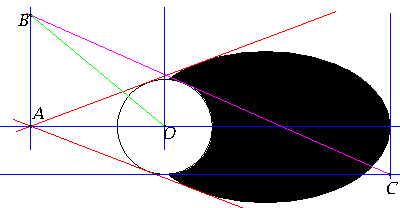
\includegraphics[width=1\linewidth]{2024-lahg-06-yl.pdf}
  \end{center}
  \vspace{-0.9cm}
\end{wrapfigure}

Joonisel (suurem koopia lisalehel) on näidatud ülaltvaates horisontaalsel laual lebav kera ja selle vari, mille heidab lauale punktvalgusallikas. Mitme kera raadiuse kaugusel kera keskpunktist asub see punktvalgusallikas? Võite teha joonisel lisakonstruktsioone ja mõõtmisi.




\hint

\solu
\begin{figure}[h]
    \centering
    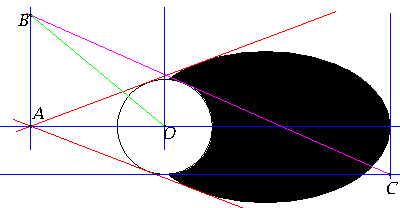
\includegraphics[width=.7\linewidth]{2024-lahg-06-sol.pdf}
\end{figure}

Lambi projektsiooni lauapinnale leiame kui ülaltvaates kera ja varju puutujate lõikepunkti $A$ (vt joonist). Tõmbame nüüd ringil horisontaalse puutuja ja vaatleme seda kui lauapinna vertikaallõike joont. Tõmbame varjule vertikaalpuutuja, selle lõikepunkt $C$ vasttõmmatud horisontaaljoonega on varju kaugeima punkti asukoht vaadeldaval vertikaallõikel. Tõmbame punktist $C$ puutuja ringjoonele ja punktist $A$ vertikaaljoone; nende lõikepunkt $B$ on lambi asukoht vertikaallõikel. Lambi kaugus vastab lõigule $OB$, joonlauaga mõõtes leiame, et see on umbes \SI{3.7}{} korda suurem, kui kera raadius.
\probend